%!TEX root = ../fys_cursus.tex

\chapter{Arbeid \& Energie}

In essentie hebben we met de wetten van Newton, de formule voor o.a. de gravitatiekracht en de kinematica voldoende om alle mechanische verschijnselen te beschrijven. Je zou dus kunnen zeggen dat we geen bijkomende elementen nodig hebben. Maar wat met het begrip energie, een fundamentele grootheid in de fysica en vaak handig bij het oplossen van probleemstellingen?  Willen we dit begrip in de mechanica gebruiken, dan zullen we het moeten defini\"eren aan de hand van begrippen die we al hebben -- zoals kracht. De wetten van Newton vormen immers het fundament van de mechanica -- alles moet hierop gestoeld zijn. 

Je leerde ooit iets over energie: \textit{een lichaam bezit energie als het de mogelijkheid heeft om arbeid te verrichten.} Zo bezit een bewegende hamer \textit{kinetische energie} omdat hij als gevolg van zijn beweging arbeid kan verrichten: hij kan een nagel in de muur drijven. De opgewonden veer
van een mechanisch horloge is een voorbeeld van \textit{potenti\"ele energie}. Als gevolg van de spanningstoestand van de veer -- die door een bepaalde plaats wordt gekarakteriseerd -- kan de veer arbeid verrichten: terwijl de veer zich geleidelijk ontspant, verricht ze arbeid door de wijzers te laten ronddraaien. %De veer verkreeg zijn potenti\"ele energie doordat degene die het horloge opwond er arbeid op leverde.

Ook in de omgangstaal kennen we de termen arbeid en energie. Je mag echter niet vergeten dat deze hier een bredere betekenis dragen dan degene die we binnen de fysica voor ogen hebben. Zo moet de \textit{kwalitatieve} omschrijving van de mogelijkheid om arbeid te verrichten, vervangen worden door een \textit{kwantitatieve}; we willen weten \textit{hoeveel} arbeid er geleverd wordt, of \textit{hoeveel} energie een bepaald lichaam bezit. Als we bovendien zeggen dat energie de mogelijkheid is om arbeid te leveren, dan moeten we in eerste instantie het begrip arbeid \textit{defini\"eren}. We gebruiken hiervoor o.a. het begrip kracht. Aan de hand van het begrip arbeid, kunnen we dan vervolgens het begrip energie defini\"eren.

\section{Arbeid geleverd door een constante kracht}

%\subsection{Kracht en verplaatsing hebben dezelfde richting}
De arbeid $W$ door een constante kracht $F$ geleverd op een lichaam bij een verplaatsing $\Delta x=x_b-x_a$ wordt gedefinieerd als \footnote{Besef dat dit een \textit{definitie} van een fysische grootheid is. Terecht zou ge u kunnen afvragen waarom we arbeid op deze manier defini\"eren en niet anders. Dat de grootheid kracht erin moet voorkomen, is duidelijk: anders kan je een veer van een horloge niet opwinden. Ook is een verplaatsing nodig om van arbeid te kunnen spreken. Als immers de veer niet beweegt, kan er geen sprake zijn van een verandering in de energietoestand van de veer en dus ook niet van een overdracht van energie naar de veer -- wat arbeid is. Dat er bijvoorbeeld geen snelheid in voorkomt, kan je inzien door je te realiseren dat de snelheid waarmee je een veer opwindt, niet mag uitmaken. Enkel de uiteindelijke toestand van de veer is van belang. En waarom dan het product van de kracht met de verplaatsing? Wel, omdat het de enige manier is waarop we aan een fysische grootheid zullen komen die de naam energie waardig is... (!). Zie hiervoor het arbeid-energietheorema.}
\begin{eqnarray}
W&=&F\Delta x
\end{eqnarray}
Hierbij moeten kracht en verplaatsing dezelfde richting hebben. De SI-eenheid van arbeid is de joule:
\begin{eqnarray*}
[W]&=&[F]\cdot[\Delta x]=\rm N\cdot m=J
\end{eqnarray*}
%\subsection{Kracht en verplaatsing; verschillende rich\-ting}
Indien de beschouwde kracht en de verplaatsing niet dezelfde richting hebben, wordt alleen de component van de kracht volgens de verplaatsing in rekening gebracht. Er is namelijk geen beweging geassocieerd met de component loodrecht op de verplaatsing.
\begin{figure}[h]
\begin{center}
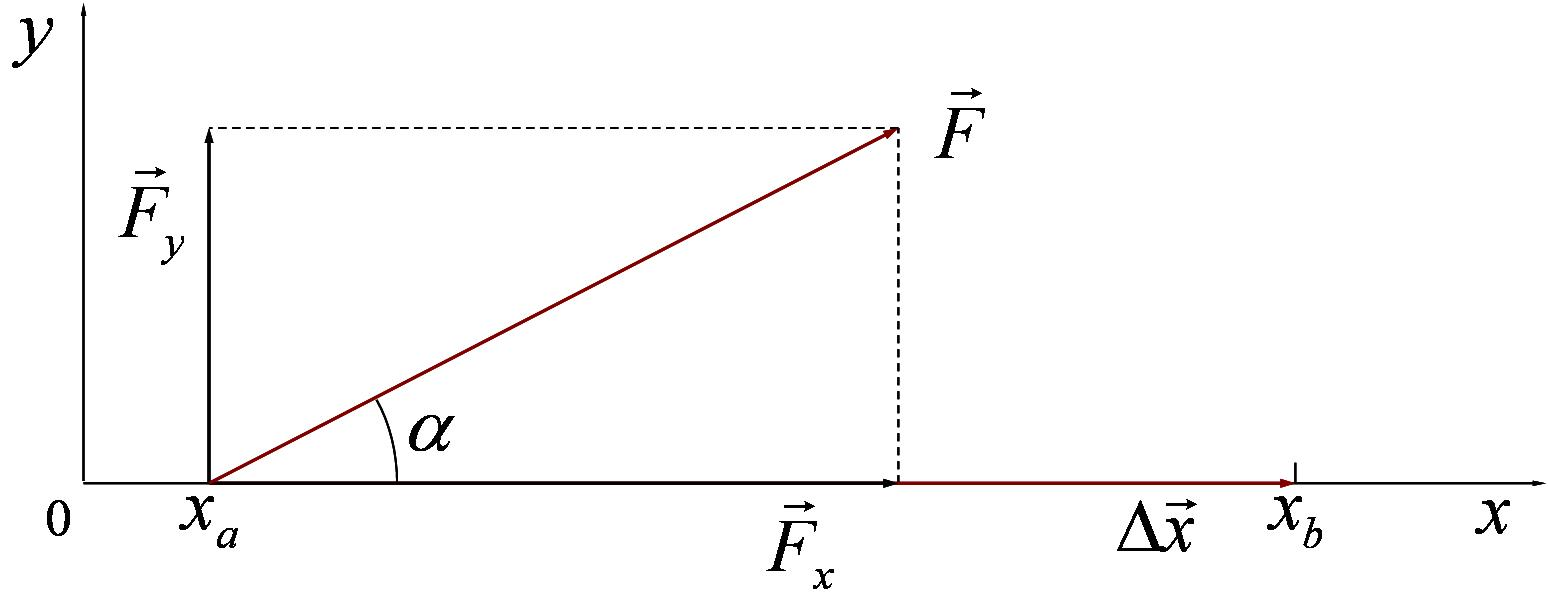
\includegraphics[width=0.7\textwidth]{arbeid_verschillende_richting}
\caption{kracht en verplaatsing met een verschillende richting}
\end{center}
\end{figure}

Als $\alpha$ de hoek tussen de kracht en de verplaatsing is, dan is de getalcomponent volgens de bewegingszin te schrijven als $F\cos{\alpha}$ en de arbeid door deze component geleverd als $W=F\cos{\alpha}\Delta x$. Dit laatste is niets anders dan het scalair product tussen de kracht en de verplaatsing.

De mechanische arbeid $W$, geleverd door een constante kracht $\vec{F}$, is gelijk aan het scalair product van de kracht met de verplaatsing:
\begin{eqnarray}
W&=&\vec{F}\cdot\Delta\vec{x}\label{def_arbeid_cste_kracht}
\end{eqnarray}

\section{Arbeid van een niet-constante kracht}

Algemeen zal een kracht gedurende de verplaatsing niet constant blijven. Ze zal met andere woorden o.a. afhankelijk zijn van de plaats waar het lichaam zich bevindt. We kunnen die afhankelijkheid beschrijven met behulp van een functie, de (grootte van de) kracht
als functie van de plaats:
\begin{eqnarray*}
F&=&F(x)
\end{eqnarray*}
Eenvoudigheidshalve beperken we ons hier tot bewegingen op een rechte. Bewegingen in meerdere dimensies vereisen een uitgebreidere integraaltheorie dan hetgeen we nu kennen.

We geven een opbouw om tot een definitie van arbeid te komen in het geval dat de kracht dus niet constant is. Ze vertoont gelijkenissen met de opbouw van de integraal.
\begin{figure}[h]
\centering
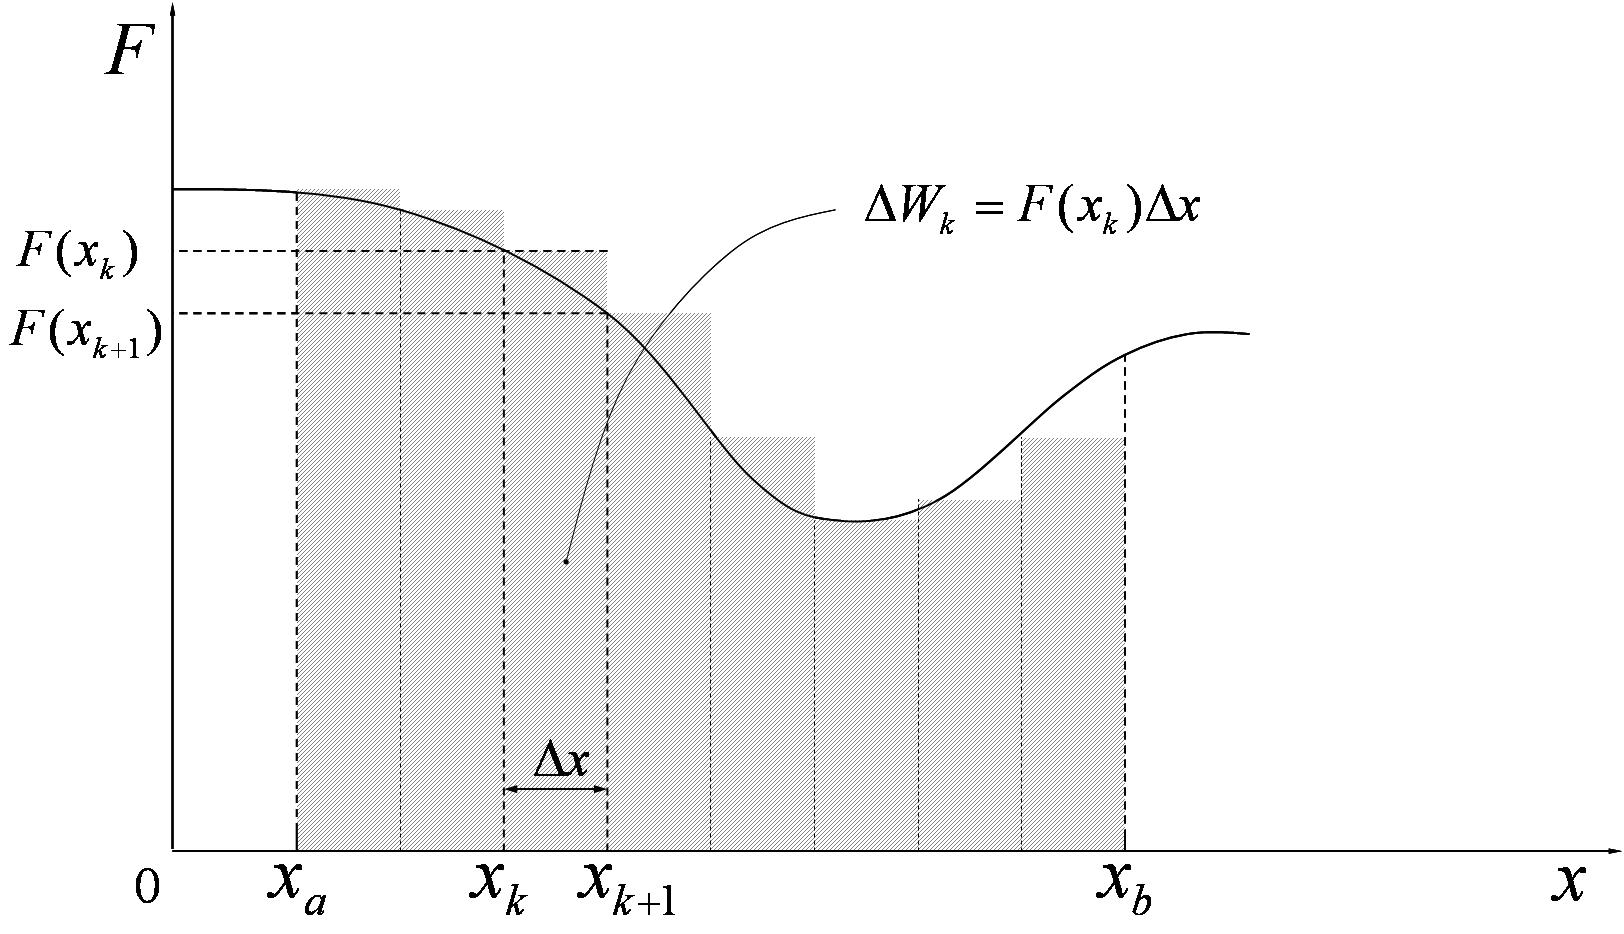
\includegraphics[width=0.85\textwidth]{arbeid_nietconstantekracht}
\caption{Opbouw arbeid bij een niet-constante kracht}
\end{figure}

Verdeel de verplaatsing $x_b-x_a$ in heel veel hele kleine stukjes $\Delta x$ bijvoorbeeld als volgt:
\begin{eqnarray*}
\Delta x&=&\frac{x_b-x_a}{n}
\end{eqnarray*}
met $n\in\mathbb{N}_0$ zeer groot. De posities tussen de stukjes kunnen we dan be\-schrij\-ven door
\begin{eqnarray*}
x_k=x_a+k\Delta x\ \ k\in\{0,1,2,\ldots,n\}
\end{eqnarray*}
Hoe kleiner $\Delta x$ is, hoe minder de kracht binnen deze stukjes vari\"eert en hoe meer dus $F(x_k)$ de kracht weergeeft die aanwezig is bij de verplaatsing van $x_{k}$ naar $x_{k+1}$. Het kleine stukje arbeid $\Delta W_k=F(x_k)\Delta x$ zouden we kunnen beschouwen als
een benadering van de geleverde arbeid gedurende deze kleine verplaatsing. De arbeid geleverd bij de gehele verplaatsing zou dan overeen kunnen komen met de som van alle stukjes geleverde arbeid. Hoe kleiner we $\Delta x$ nemen hoe meer die som overeenkomt met wat de totale arbeid zou moeten zijn, vandaar dat in de limiet van $\Delta x$ gaande naar nul, we de geleverde arbeid zouden kunnen vinden. Deze limiet komt overeen met het nemen van een integraal:
\begin{eqnarray*}
W\,=\,\lim_{\Delta x\rightarrow0}\sum_{k=0}^{n-1}\Delta W_k
%&=&\lim_{n\rightarrow\infty}\sum_{k=0}^{n-1}F(x_k)\Delta x\\
\,=\,\lim_{n\rightarrow\infty}\sum_{k=0}^{n}F(x_k)\Delta x
\,=\,\int_{x_a}^{x_b}F(x)~dx
\end{eqnarray*}
Dit moet de volgende algemene definitie van arbeid legitimeren.

\kader{De mechanische arbeid $W$, geleverd door een kracht $\vec{F}(x)$ gedurende de verplaatsing op een rechte van $x_a$ tot $x_b$ wordt gedefinieerd als
\begin{eqnarray}\label{W}
W=\int_{x_a}^{x_b}F_x(x)\ dx
\end{eqnarray}
waarbij $F_x(x)$ de getalcomponent van $\vec{F}(x)$ is volgens de bewegingsrichting.}

\textit{Opmerkingen:}
\begin{enumerate}
\item[-]Indien de kracht als functie van de plaats expliciet gekend is, kan de integraal verder bepaald worden.
\item[-]De twee vorige definities zijn speciale gevallen van deze definitie. Inderdaad bekomen we de formule (\ref{def_arbeid_cste_kracht}) indien de kracht een constante is. De kracht schuift voor het integraalteken en de integraal zelf wordt de verplaatsing.\footnote{Ga dit na!}
\item[-]Arbeid kan negatief zijn. Dit is o.a. het geval wanneer kracht en verplaatsing een tegengestelde zin hebben.
\end{enumerate}

\label{voorbeeld Hooke}
\voorbeeld{Arbeid door een veer geleverd}{\textsf{Een eenvoudig maar duidelijk voorbeeld van een kracht die afhankelijk is van de plaats is de kracht door een veer uitgeoefend. Voor niet te grote uitwijkingen wordt deze gegeven door de wet van Hooke:}
\begin{eqnarray*}
F(x)=-kx
\end{eqnarray*}
\textsf{Hierin is $k$ de veerconstante en $x$ de verlenging van de veer t.o.v. zijn evenwichtspositie~\footnote{Uit het vierde jaar ken je deze uitdrukking onder de vorm $F=k\Delta l$.}. Het minteken komt van het feit dat de kracht steeds tegengesteld is aan de uit\-wij\-king. Het is een \textit{terugroepkracht}. Bij het samendrukken van de veer bijvoorbeeld is $x<0$ zodat de kracht positief en dus tegengesteld aan de uitwijking is.}
\begin{figure}[h]
\centering
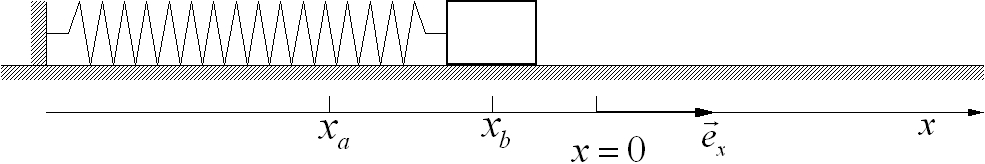
\includegraphics[width=0.85\textwidth ,angle=0]{elastische_energie}
\end{figure}

\textsf{We willen de arbeid berekenen door de veerkracht geleverd op een massa bij de verplaatsing van een verlenging $x_a$ naar een verlenging $x_b$. Volgens de definitie wordt dit:}
\begin{eqnarray*}
W\,=\,\int_{x_a}^{x_b}F(x)~dx&=&\int_{x_a}^{x_b}-kx~dx\\
&=&-k\left[\frac{x^2}{2}\right]_{x_a}^{x_b}\\
&=&\frac{1}{2}k{x_a}^2-\frac{1}{2}k{x_b}^2
\end{eqnarray*}
\textsf{Indien het beginpunt $x_a$ verder uit de evenwichtspositie ligt dan het eindpunt $x_b$ is de geleverde arbeid positief.}}

%\section{Vermogen}
%Dit onderdeel hoef je niet te kennen.
\section{Het arbeid-energietheorema}

Indien op een voorwerp een resulterende kracht inwerkt, moet de snelheid ervan veranderen. Volgens de tweede wet van Newton krijgt het immers een versnelling. Indien kracht en verplaatsing dezelfde zin hebben, is er een snelheidstoename en is de arbeid door de kracht geleverd positief. Er moet dus misschien een verband bestaan tussen de geleverde arbeid en de verandering in snelheid \ldots 

\kader{\textit{Het arbeid-energietheorema}

Voor de arbeid door de \textit{resulterende kracht} op een voorwerp geleverd geldt:
\begin{eqnarray}
W=\int_{x_a}^{x_b}F(x)\
dx=\frac{mv_b^2}{2}-\frac{mv_a^2}{2}\nonumber
\end{eqnarray}
waarin $m$ de massa van het voorwerp is en $v_a$ en $v_b$ de snelheden van het voorwerp op respectievelijk het begin- en het eindpunt.

In het rechterlid verschijnt een grootheid die we \textit{defini\"eren} als de \mbox{\textit{kinetische energie}} van het voorwerp:
\begin{eqnarray}
E_k&=&\frac{mv^2}{2}\nonumber
\end{eqnarray}
De arbeid geleverd door de resulterende kracht op een voorwerp, is dus gelijk aan het verschil van de kinetische energie van het lichaam in begin- en eindpunt:
\begin{eqnarray}
W&=&E_{k,b}-E_{k,a}
\end{eqnarray}}

\textit{Opmerkingen:}
\begin{enumerate}
\item[-]Dit theorema geeft een samenhang tussen arbeid en energie
zoals we dat verwachten. De \textit{nettoarbeid} geleverd over het hele traject \textit{door} de resulterende kracht \textit{op} het voorwerp, resulteert in een toe- of afname van de
kinetische energie van dat voorwerp met \textit{eenzelfde waarde}.
Zoveel arbeid als geleverd wordt, zoveel energie krijgt of verliest het voorwerp. De manier waarop de arbeid is geleverd tussen begin- en eindpunt speelt geen rol. Enkel de totale hoeveelheid is van belang.
%\footnote{Indien een kracht arbeid zou leveren als ze
%loodrecht op de verplaasting zou staan, dan zou er arbeid kunnen zijn
%\textit{zonder} een toename in snelheid. M.a.w. zou dit theorema dan
%niet opgaan. De betekenis van arbeid zou dan verloren gaan.}

\item[-]Indien de geleverde nettoarbeid op een voorwerp positief is, neemt de
kinetische energie toe. Voor positieve arbeid hebben kracht en
verplaatsing tussen begin- en eindpunt meer eenzelfde dan een
tegengestelde zin zodat de snelheid inderdaad kan toenemen. Denk bijvoorbeeld aan een vallende steen; hier levert de zwaartekracht ook positieve arbeid.
\item[-]Indien de geleverde nettoarbeid op een
voorwerp negatief is, neemt de kinetische energie af. Voor een
negatieve arbeid hebben kracht en verplaatsing tussen begin- en
eindpunt meer een tegengestelde dan een gelijke zin. De snelheid zal op die manier kunnen afnemen. De geleverde arbeid op
bij\-voor\-beeld een hamer die een nagel in de muur drijft, is
negatief. Zijn snelheid, en dus zijn kinetische energie, is
afgenomen. Ze is gebruikt om de nagel in de muur te krijgen.
Inderdaad is de kracht \textit{door} de hamer op de nagel
uitgeoefend met de beweging mee (de \textit{hamer} levert positieve arbeid, en verliest energie) en is de reactiekracht, de kracht door de nagel \textit{op} de hamer uitgeoefend, tegengesteld
aan de beweging (de \textit{nagel} levert negatieve arbeid, of ontvangt dus energie).
\item[-]Merk op dat dit theorema geldt voor de arbeid door de
\textit{resulterende kracht} geleverd en in de regel niet door
slechts \'e\'en van de krachten die op het voorwerp werken. Het is
de resulterende kracht die voor een resulterende versnelling van het
lichaam zorgt en dus voor een verandering in de snelheid.
\end{enumerate}

\textit{Bewijs arbeid-energietheorema}

Veronderstel dat de resulterende kracht wordt gegeven door de functie $F(x)$. We berekenen de arbeid door de resulterende kracht geleverd wanneer het voorwerp een verplaatsing ondergaat van $x_a$ naar $x_b$ door de tweede wet van Newton te gebruiken\footnote{Het gaat hier immers over de resulterende kracht\ldots}, de kettingregel en een substitutie door te voeren.
\begin{eqnarray*}
W&=&\int_{x_a}^{x_b}F(x)dx\\
&=&\int_{x_a}^{x_b}ma\,dx\\
&=&\int_{x_a}^{x_b}m\frac{dv}{dt}dx
\end{eqnarray*}
Door de kettingregel $\frac{dv}{dt}=\frac{dv}{dx}\frac{dx}{dt}$ en de definitie van snelheid $v=\frac{dx}{dt}$ te gebruiken, krijgen we
\begin{eqnarray*}
W&=&\int_{x_a}^{x_b}m\frac{dv}{dx}\frac{dx}{dt}dx\\
&=&\int_{x_a}^{x_b}m\frac{dv}{dx}v\,dx\\
\end{eqnarray*}
Deze integraal kunnen we uitwerken door de substitutie $v=v(x)$ door te voeren\footnote{Omdat de substitutie met de letter $v$ enigszins verwarrend is, vind je onder de uitdrukking de benoeming van de variabelen zoals je die voor de substitutieregel kent, nl. met $u$. En hopelijk overbodig, hier de substitutieregel:
\begin{eqnarray*}
\int_{a}^{b}f(\underbrace{g(x)}_u)\underbrace{\underbrace{g'(x)}_{u'}\underbrace{dx}_{dx}}_{du}=\int_{g(a)}^{g(b)}f(u)du
\end{eqnarray*}}. De integratiegrenzen $x_a$ en $x_b$ voor de positie $x$, worden $v_a=v(x_a)$ en $v_b=v(x_b)$ voor de snelheid $v$. We wisselen voor de duidelijkheid ook twee factoren om.
\begin{eqnarray*}
W&=&\int_{x_a}^{x_b}m\underbrace{v\frac{dv}{dx}\,dx}_{u\cdot u'\,dx}\\
&=&\int_{v(x_a)}^{v(x_b)}mv\,dv\\
&=&\left[\frac{mv^2}{2}\right]_{v_a}^{v_b}\\
&=&\frac{mv_b^2}{2}-\frac{mv_a^2}{2}
\end{eqnarray*}
\phantom{}\hfill$\blacksquare$

\voorbeeld{Opgave arbeid-energie theorema}{\textsf{ Een horizontaal liggende veer op tafel heeft een veerconstante $k=360\rm\,N/m$ en wordt $11,0\rm\,cm$ ingedrukt. Een blok van $1,85\rm\,kg$ wordt tegen de gespannen veer gelegd en losgelaten. De wrijvingsco\"effici\"ent tussen het blok en de tafel is $0,38$.
\begin{enumerate}
\item Hoeveel arbeid levert de veerkracht vanaf de ingedrukte toestand tot in zijn evenwichtstoestand?
\item Hoeveel arbeid levert de wrijvingskracht over hetzelfde traject?
\item Hoe groot is de nettoarbeid?
\item Welke snelheid heeft het blok wanneer het zich, in de evenwichtstoestand, van de veer losmaakt?
\end{enumerate}
}}

%\newpage

\section{Potenti\"ele energie}

Naast kinetische energie -- de energie geassocieerd met de beweging van een lichaam -- kunnen we een andere vorm van mechanische energie defini\"eren: de \textit{potenti\"ele energie}. Dit is de energie geassocieerd met de plaats of configuratie van een lichaam. Een lichaam met kinetische energie heeft energie omdat het als gevolg van zijn beweging arbeid kan verrichten op een ander object. Kan een object arbeid verrichten als gevolg van zijn plaats, dan noemen we deze energie potenti\"ele energie.

Het leveren van arbeid op een voorwerp hoeft niet altijd te resulteren in een verandering van de kinetische energie. Bijvoorbeeld wanneer de arbeid van slechts \'e\'en van de krachten op een voorwerp wordt beschouwd en niet de arbeid door de resulterende kracht geleverd. De geleverde arbeid moet dan naar een andere vorm van energie gaan: potenti\"ele energie. Bij het opwinden van een horloge bijvoorbeeld wordt de geleverde arbeid gebruikt om de veer samen te drukken. De veer kan zich daarna ontspannen en arbeid op de wijzers leveren.

De vraag \textit{hoeveel} energie een voorwerp heeft, zal bij nader inzien enkel relatief kunnen worden bepaald. Is bijvoorbeeld de kinetische energie van een bekertje koffie op het tafeltje van de trein van Brussel naar Gent gelijk aan nul omdat het t.o.v. het tafeltje niet beweegt? Of is de kinetische energie verschillend van nul omdat het bekertje een snelheid heeft t.o.v iemand buiten de trein en dus, moest de trein plots stoppen, het bekertje verder zal vliegen en (veel opkuis-) arbeid kan leveren? En hoeveel energie heeft een blokje op een bepaalde hoogte? Zoveel als dat het arbeid kan leveren? Dat zal niet eenduidig te bepalen zijn. De geleverde arbeid tot op het tafeloppervlak, de grond of de bodem van de put die we vervolgens hebben gegraven is steeds verschillend. De geleverde arbeid, en dus de energie, is afhankelijk van het referentiepunt dat we nemen. In ieder geval moet de energie van een voorwerp afnemen met de hoeveelheid arbeid die het levert.

%Potenti\"ele energie is echter niet in alle gevallen te
%defini\"eren. In namelijk niet alle gevallen is de mogelijk te
%leveren hoeveelheid arbeid eenduidig bepaald.

%\newpage

\subsection{Elastische potenti\"ele energie}\label{elastische
potentiele energie}

We hernemen het voorbeeld van de veerkracht (\ref{voorbeeld Hooke}).
\begin{figure}[h]
\begin{center}
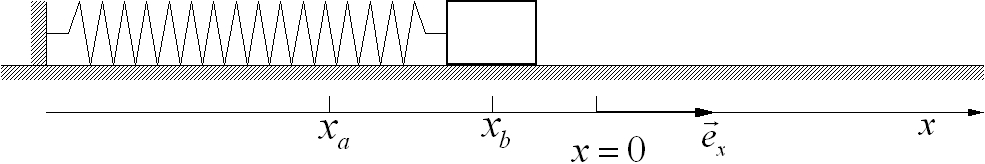
\includegraphics[width=0.8\textwidth ,angle=0]{elastische_energie}
\end{center}
\end{figure}
\newline
Hier vonden we dat de hoeveelheid arbeid door de veerkracht geleverd
bij een verplaatsing van $x_a$ naar $x_b$ gegeven wordt door:
\begin{eqnarray*}
W&=&\frac{1}{2}kx_ a^2-\frac{1}{2}kx_ b^2
\end{eqnarray*}
De geleverde arbeid kan geschreven worden als het verschil van de uitdrukking $\frac{1}{2}kx^2$ ge\"evalueerd in begin- en eindpunt. De waarde van de uitdrukking neemt af met de hoeveelheid arbeid die is geleverd. We kunnen de uitdrukking dus interpreteren als de hoeveelheid energie die de veer op een bepaald punt, een bepaalde plaats, bezit. Dat wat immers verloren gaat aan energie -- de oorspronkelijke energie min de overblijvende energie -- moet door de veer worden geleverd als arbeid. We noemen de uitdrukking de \textit{elastiche potenti\"ele energie} van een veer:
\begin{eqnarray}
E_p&=&\frac{1}{2}kx^2\label{Ep=1/2kx^2}
\end{eqnarray}
De geleverde arbeid kunnen we vervolgens schrijven als
\begin{eqnarray*}
W&=&E_{p,a}-E_{p,b}\,=\,-(E_{p,b}-E_{p,a})\\
&\Updownarrow&\\
W&=&-\Delta E_p
\end{eqnarray*}
Hierin is $\Delta E_p$ de verandering van potenti\"ele energie: $\Delta E_p=E_{p,\rm eind}-E_{p,\rm begin}$. Als de veer arbeid verricht dan gaat dat ten koste van haar potenti\"ele energie: is de geleverde arbeid $W$ positief, dan moet er een afname van de potenti\"ele energie zijn (de verandering $\Delta E_p$ moet negatief zijn). Opnieuw: de hoe\-veel\-heid geleverde arbeid komt overeen met het verlies in potenti\"ele energie tussen begin- en eindpunt. Is de verandering van de potenti\"ele energie $\Delta E_p$ positief dan is de geleverde arbeid negatief. Negatieve arbeid betekent dat i.p.v. het leveren van arbeid (het weggeven van energie), er van elders energie wordt toegevoegd en wordt omgezet in potenti\"ele energie.

\subsection{Gravitationele potenti\"ele energie}\label{gravitationele potentiele energie}

Beschouw een massa op een hoogte boven het aardoppervlak. Vanuit deze positie kan ze arbeid verrichten en zal ze dus potenti\"ele energie bezitten. Als we de massa bijvoorbeeld laten vallen kan ze op de grond een nagel inslaan en dus arbeid verrichten.
\begin{figure}[h]
\begin{center}
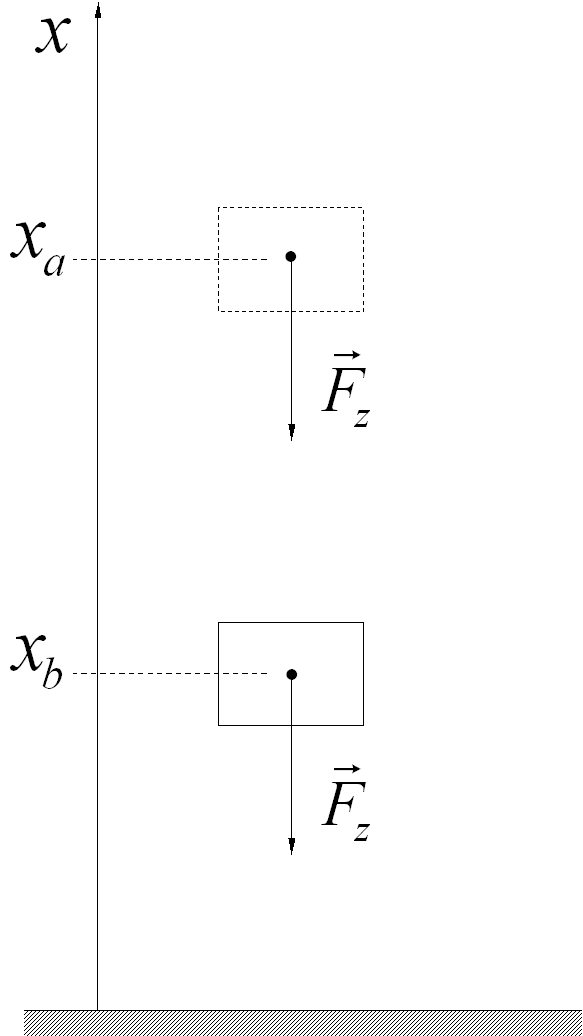
\includegraphics[height=5.5cm ,angle=0]{gravitationele_energie}
\end{center}
\end{figure}
Bij het vallen van een hoogte $x_a$ naar een hoogte $x_b$ levert de zwaartekracht die aan de massa trekt een arbeid gelijk aan:
\begin{eqnarray*}
W\,=\,\int_{x_a}^{x_b}F_zdx\,=\,\int_{x_a}^{x_b}(-mg)dx\,=\,mgx_a-mgx_b
\end{eqnarray*}
Hier voldoet de uitdrukking $mgx$ aan wat we verwachten van potenti\"ele ener\-gie. Het verschil van de uitdrukking ge\"evalueerd in het beginpunt en het eindpunt -- het verschil in energie -- is gelijk aan de hoeveelheid arbeid die tussen deze twee posities kan worden geleverd. We noemen de uitdrukking de \textit{gravitationele potenti\"ele energie}. En als we $x$ door $h$ vervangen, krijgen we de gekende vorm:
\begin{eqnarray}
E_p&=&mgh\label{Ep=mgh}
\end{eqnarray}
Net zoals bij de veerkracht geldt $W=-\Delta E_p$. 

Waarom nu eigenlijk dat minteken? Als de massa valt, wordt door de zwaartekracht positieve arbeid verricht. Op een punt iets lager dan waar de massa was vertrokken, kan de massa nog minder ver vallen zodat ze vanuit dit punt minder arbeid kan leveren. Haar potenti\"ele energie is afgenomen of de verandering $\Delta E_p$ is negatief. Dat wat aan potenti\"ele energie verloren is gegaan, is aan arbeid geleverd. Als de massa omhoog wordt gegooid, heeft ze in een punt hoger dan daar waar ze vertrok meer potenti\"ele energie. Vanaf een grotere hoogte kan ze meer arbeid leveren. De potenti\"ele energie neemt dus toe of de verandering $\Delta E_p$ is positief. De zwaartekracht $F_z$ is echter tegengesteld (naar beneden gericht) aan de verplaatsing (naar boven) zodat de geleverde arbeid negatief is. Het toenemen van de energie kan maar mogelijk zijn als van elders energie aan de massa wordt gegeven. In dit geval is ze afkomstig van de kinetische energie die bij het opwerpen wordt meegegeven.

Merk op dat de massa in staat is arbeid te verrichten als gevolg van het feit dat de zwaartekracht erop inwerkt en de massa bijgevolg \textit{zelf} een even grote kracht kan uitoefenen. Op die manier kunnen we de potenti\"ele energie toekennen aan de massa; \textit{de massa} gaat op deze manier in staat zijn arbeid te verrichten.

\subsection{Gravitationele potenti\"ele energie, algemeen}\label{gravitationele potentiele energie alg}

Beschouw een massa onderhevig aan de universele gravitatiekracht. We gaan opnieuw opzoek naar een potenti\"ele energiefunctie geassocieerd aan deze kracht.
\begin{figure}[h]
\begin{center}
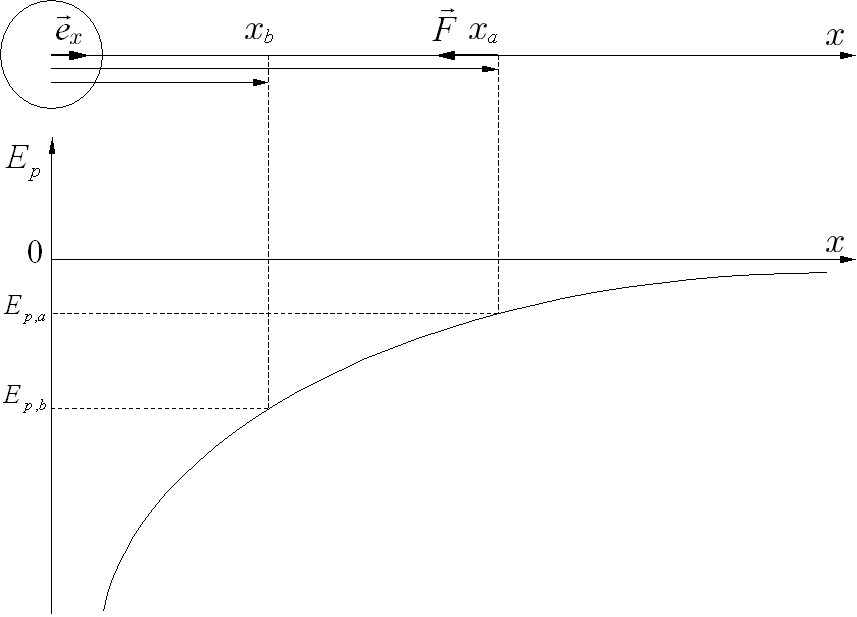
\includegraphics[width=0.9\textwidth ,angle=0]{gravitationele_energie_algemeen}
\end{center}
\end{figure}

Kiezen we een $x$-as met de oorsprong op de massa $m$ dan wordt, omdat de kracht steeds naar de oorsprong is gericht, de component van de universele gravitatiekracht op de massa $m'$ gegeven door
\begin{eqnarray*}
F(x)&=&-G\frac{mm'}{x^2}
\end{eqnarray*}
De arbeid die door de gravitatiekracht wordt geleverd bij de verplaatsing van de massa $m'$ van $x_a$ naar $x_b$ wordt dan:
\begin{eqnarray*}
W&=&\int_{x_a}^{x_b}-G\frac{mm'}{x^2}~{\rm d}x\\
&=&-Gmm'\int_{x_a}^{x_b}\frac{1}{x^2}~{\rm d}x\\
&=&-Gmm'\left[-\frac{1}{x}\right]_{x_a}^{x_b}\\
&\Updownarrow&\\
W&=&\left(-G\frac{mm'}{x_a}\right)-\left(-G\frac{mm'}{x_b}\right)
\end{eqnarray*}
De potenti\"ele energie voor een massa $m'$ wordt bijgevolg geven
door
\begin{eqnarray}
E_p&=&-G\frac{mm'}{x}\label{Ep=-Gmm'/x}
\end{eqnarray}

\subsection{Referentiepunt van de potenti\"ele energie}

Ai, de potenti\"ele energiefunctie (\ref{Ep=-Gmm'/x}) is voor alle waardes van $x$
\textit{negatief}. Zou potenti\"ele energie overeenkomen met de mogelijk te leveren hoeveelheid  arbeid, dan zou de massa met andere woorden minder dan geen arbeid kunnen leveren vanop een
bepaalde afstand. Een vallende steen op de aarde lijkt toch wel het tegendeel te bewijzen\ldots. Bovendien is de hoeveelheid arbeid die de massa $m'$ vanaf een bepaald punt tot aan $m$ kan leveren \textit{oneindig} groot \footnote{Waarom?}. De massa zou dus oneindig veel energie hebben. Zeggen dat de potenti\"ele energie gelijk is aan de hoeveelheid arbeid die kan worden verricht, is dus niet mogelijk?!

De potenti\"ele energie kan niet als een absolute maar enkel als een relatieve grootheid worden gedefinieerd. Het enige wat we van de potenti\"ele ener\-gie kunnen verwachten is dat het
\textit{verschil} tussen een begin- en eindpunt overeenkomt met de hoeveelheid geleverde arbeid tussen die twee punten.
%\begin{eqnarray*}
%W&=&-\Delta E_p
%\end{eqnarray*}
Een relatieve grootheid is tot op een constante na bepaald. Het gevolg is dat als $E_p$ een potenti\"ele energiefunctie is, $E_p'=E_p+\rm cte$ dat ook is. Immers:
\begin{eqnarray*}
E_{p,a}'-E_{p,b}'&=&(E_{p,a}+{\rm cte})-(E_{p,b}+{\rm cte})\\
&=&E_{p,a}-E_{p,b}\\
&=&W
\end{eqnarray*}
Bij de potenti\"ele energiefuncties (\ref{Ep=1/2kx^2}), (\ref{Ep=mgh}) en (\ref{Ep=-Gmm'/x}) zoals we ze hiervoor hebben gegeven, mag dus steeds een constante worden opgeteld. Het
\textit{re\-fe\-ren\-tiepunt} -- daar waar de potenti\"ele energie nul is -- kan vrij worden gekozen.

\subsection{Potenti\"ele energie}

Uit de drie voorbeelden blijkt dat in het algemeen de potenti\"ele
energie een plaatsafhankelijke functie moet zijn waarvan het
verschil tussen twee punten overeenkomt met de geleverde arbeid door
de kracht geassocieerd met deze functie. Noemen we deze functie
$U(x)$, dan moet gelden:
\begin{eqnarray*}
  W=\int_{x_a}^{x_b}F(x)~{\rm d}x &=&-(U(x_b)-U(x_a))\\
  &\Updownarrow&\\
  \int_{x_a}^{x_b}-F(x)~{\rm d}x &=&U(x_b)-U(x_a)\\
\end{eqnarray*}
Als $U(x)$ een primitieve functie voor $-F(x)$ is (dus een functie
waarvan de afgeleide de functie $-F(x)$ is: $U'(x)=-F(x)$) dan is
aan deze voorwaarde voldaan. Immers geldt dan:
\begin{eqnarray*}
\int_{x_a}^{x_b}-F(x)~{\rm d}x=\int_{x_a}^{x_b}\frac{d}{dx}U(x)~{\rm d}x&=&U(x_b)-U(x_a)\\
\end{eqnarray*}
Algemeen geldt dan ook voor de potenti\"ele energie:

\kader{Indien er voor een plaatsafhankelijke kracht $F(x)$ een functie $U(x)$ bestaat
waarvoor de afgeleide op een minteken na de kracht is,
\begin{eqnarray}\label{U(x)}
F(x)&=&-\frac{d}{dx}U(x)\nonumber
\end{eqnarray}
dan wordt $U(x)$ de \textit{potenti\"ele energie} genoemd.}

De potenti\"ele energie is dus een functie waarvoor de negatieve afgeleide de kracht is. Waarom een minteken? Een positieve afgeleide betekent een toename van de potenti\"ele energie. Om naar een hogere energie te gaan moet \textit{tegen} de kracht in worden bewogen. De kracht moet dus tegengesteld zijn aan de richting waarin de potenti\"ele enrgie toeneemt.

Zie ook dat de potenti\"ele energie inderdaad tot op een constante na is ge\-de\-fi\-ni\-eerd. Bij het afleiden valt immers een constante weg.

Een kracht waarvoor een potentiaalfunctie bestaat, levert arbeid die enkel bepaald wordt door begin- en eindpunt. De arbeid is dus onafhankelijk van de gevolgde weg. Zo'n kracht wordt conservatief genoemd. Enkel voor conservatieve krachten bestaat dus een potenti\"ele energie.

Ga na dat de energiefuncties die we bij de drie voorbeelden (\ref{gravitationele potentiele energie}), (\ref{elastische potentiele energie}) en (\ref{gravitationele potentiele energie
alg}) vonden, voldoen aan deze definitie en dus potenti\"ele energiefuncties zijn.

%\newpage

\section{Het beginsel van behoud van energie}\label{beginsel_behoud_energie}

Het arbeid-energietheorema relateert de geleverde arbeid door een resulterende kracht met de toename aan kinetische energie. Het zegt dat de hoeveelheid geleverde arbeid door de resulterende kracht volledig wordt gebruikt voor de toename van kinetische energie.
Anderzijds als met de resulterende kracht een potenti\"ele energie kan worden geassocieerd, dan is de geleverde arbeid afkomstig van het verlies in potenti\"ele energie. De energie die dus onder de vorm van potenti\"ele energie verloren gaat wordt in kine\-ti\-sche energie gewonnen. En dit zodanig dat de som van beide energi\"en - de totale mechanische energie - constant blijft.
\newline
\newline
Uit $W=\Delta E_k$ en $W=-\Delta E_p$ volgt:
\begin{eqnarray}
\Delta E_k&=&-\Delta E_p\nonumber\\
%&\Updownarrow&\nonumber\\
%E_{k,b}-E_{k,a}&=&E_{p,a}-E_{p,b}\nonumber\\
&\Updownarrow&\nonumber\\
E_{k,a}+E_{p,a}&=&E_{k,b}+E_{p,b}\nonumber
\end{eqnarray}
Spelen dus enkel krachten een rol waarvoor een potenti\"ele energie functie bestaat, dan is de som van de kinetische en de potenti\"ele energie van een voorwerp gedurende de beweging constant.

\kader{\textit{Het beginsel van behoud van mechanische energie}
\begin{eqnarray}
E_{k,a}+E_{p,a}&=&E_{k,b}+E_{p,b}\\
&\Updownarrow&\nonumber\\
E=\frac{mv^2}{2}+E_p~&=&~\mathrm{constant}
\end{eqnarray}\vspace{0cm}}

Het principe van behoud van energie is een van de meest fundamentele principes in de fysica \ldots 

%\clearpage
%\newpage
